\documentclass[a4paper, 12pt]{article}

\usepackage[margin=1in]{geometry}
\usepackage{graphicx}
\usepackage[english]{babel}
\graphicspath{ {./images/} }

\renewcommand{\baselinestretch}{2}

\usepackage{fancyhdr}
\usepackage{dirtytalk}
\pagestyle{fancy}



\usepackage{amsthm}
\usepackage{amssymb}
\usepackage{listings}
\lstset{
    basicstyle = \small \ttfamily,
    columns = fullflexible,
    breaklines = true,
    numbers = left,
    stepnumber = 1,
    showstringspaces = false,
    tabsize = 1}


\lhead{Dustin Powell}
\chead{Senior Project v1.20}
\rhead{4/23/2020}

\linespread{1.75}
\title{Predicting  A Personality Trait Using A Machine Learning Algorithm}
\date{Spring 2020}
\author{Dustin Powell \\IT 451 - 01 Senior Capstone}

\begin{document}
\pagenumbering{roman}

\newtheorem*{theorem}{Primary Question}
\maketitle

\begin{abstract}
A study by the Proceedings of the National Academy of Sciences of the United States of America (PNAS) shows that using statistics personality traits of a person can be predicted. The PNAS study inspired a machine learning algorithm to be made to show that the personality trait of an individual is predictable by only using only one feature and a multilayer perceptron classifier within the scikit--learn library using Python 3. The code shows that making simple changes to the estimators of scikit--learn's multilayer perceptron classifier can yield high overall average accuracy scores at the expense of time.  The research that leads up to the creation of the algorithm shows that the field of machine learning is very expansive and overlaps with other disciplines such as statistics, mathematics, and biology and that many fine details go into making a machine learning algorithm work.
\end{abstract}
\newpage

\tableofcontents
\newpage

%-------------------------------------------------------------------------------
\pagenumbering{arabic}

\setcounter{page}{1}

\section{Introduction}
\begin{paragraph}
\indent According to Our World In Data, 3.5 billion people use the internet with about 2.3 billion internet using the social network Facebook\textsuperscript{\textregistered} \cite{IntStats}. The number of people that are using the internet is not slowing down but snowballing, as in the past few years, about 640,000 new people access the internet daily \cite{IntStats}. As more people become connected, a lot more of people's \say{information} is becoming publicly viewable compared to before the creation of the internet. Given that this abundance of information being available, what about all of the private information that people want to keep secret? Using machine learning, much of this data can be used for predicting information about an individual. One question arises on how much information about an individual is needed to make an accurate prediction about a person's traits? The purpose of this work is to use online data to demonstrate that using a limited amount of information can lead to uncovering private details about an individual. Using the online data and machine learning shows that very little information is required to make an accurate prediction on an individuals information. In 2013, an article published by the Proceedings of the National Academy of Sciences of the United States of America (PNAS) provides an insight of using statistics and the likes of users on a social media platform to predict the user's private information such as age, race, political views, and other personnel information \cite{Kosinski2013}.
\end{paragraph}

\subsection{Prediction of Private Information}
\begin{paragraph}
\indent The post--liking habits of 58,466 people were used to predict various private aspects about the user, such as age, race, intelligence, and political views \cite{Kosinski2013}. The data collected had an overall average of 170 likes per user \cite{Kosinski2013}. The study consisted of three steps to make predictions, consisting of two phase of organizing data and the final stage using \textit{logistic and linear regression} functions to make predictions \cite{Kosinski2013}. The steps in order can be found in Fig. 1 outlining the steps taken to predict an individual's information.  
\par
\indent In the first step, the researchers assembled the users' data into a matrix called a \say{user--like matrix}, portrayed in Fig. 1, shows each of post that a user based on topic or specific subject \cite{Kosinski2013}. \textit{Singular Value Decomposition} was then used on the set of data and then assembled into a \say{user--components matrix}, which then used with linear and logistic regression functions to determine the private attributes of the individual \cite{Kosinski2013}. The results of the case study concluded that by using linear and logistic regression along with other sets of data like web browsing information can be used to determine various private aspects about the person \cite{Kosinski2013}. Certain individual traits of the users', such as ethnicity, were able to be validated based upon the profiles that the users have created \cite{Kosinski2013}. The results of the study have raised ethical questions as an unauthorized individual could cause a person to come into harm's way if within a culture that personality or habit that is not tolerated \cite{Kosinski2013}.

\begin{figure}[ht]
\centering
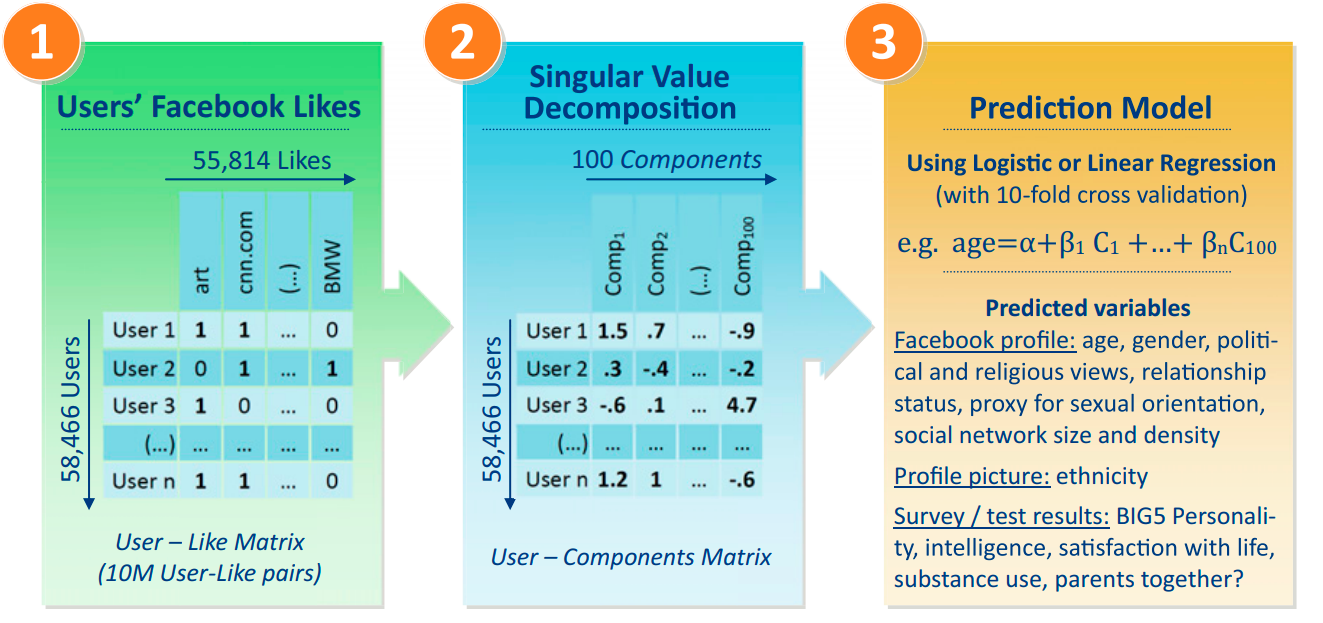
\includegraphics[scale=0.30]{PNAS}
\caption{The process from the papers of the PNAS study outlining the steps used to make predictions with Facebook\textsuperscript{\textregistered} data \cite{Kosinski2013}.}
\end{figure}

\end{paragraph}

\subsection{Question To Address And Project Goal}
\begin{paragraph}
\indent The concept of predicting people's private information is very alarming as if the wrong people access the information about an individual, it can be misused to harm that individual. The alarming and possible harmful implications of the PNAS study prompts the following question.
\begin{theorem}
Using a machine--learning algorithm what is the minimum amount of information needed to predict the personality trait of a given person accurately?
\end{theorem}
Within the PNAS article, people's information can be predicted, but can information be predicted accurately with little data. The idea leads to the hypothesis that a personality trait of a given person is predictable with one feature, an overall average accuracy score of 90 percent or higher can be obtained, and the overall accuracy will increase as features in the models increase. Before constructing an experiment to analyze the question fully. Basic information about \textit{analytics}, statistics, and machine learning is necessary before diving into the code and estimators used for machine learning and code testing the question.
\end{paragraph}

%-------------------------------------------------------------------------------
\section{Predictive Analytics}
\subsection{Big Data's Relationship With Predictive Analytics}
\begin{paragraph}
\indent The case study conducted by Kosinski, Stillwell, and Gaepel (2013) reflects an overarching concept of a bigger project at hand called \textit{big data}. Data generated from users by visiting websites, liking posts, and watching videos is stored into large databases \cite{Jeble2016}. The databases are located in warehouses full of computers called servers with a range of purposes such as delivering data to web pages, mathematical research, and storage of digital information \cite{Jeble2016}. Companies such as Google\textsuperscript{\textregistered}, Amazon\textsuperscript{\textregistered}, and Facebook\textsuperscript{\textregistered}
use these massive amounts of data as a way to make predictions about the users to help enhance the experience on their platforms \cite{Jeble2016}. The scale of the data generated within a couple of hours can be numerous terabytes or up to a few petabytes of data \cite{Jeble2016}. Where a petabyte equals to $1*10^{-9}$ megabytes of information. All this data is stored to look for relationships between all of the collected information \cite{Jeble2016}. The data is collected and sorted into three different types of data, structured, unstructured, and semi-structured \cite{Jeble2016}. Structured data is any data collected from sales, batch process, and systems like customer--relationship management systems \cite{Jeble2016}. Structured data is clearly understood, defined, and can immediately be stored in databases  \cite{Jeble2016}. The second type of information is called unstructured data that comes from social media, emails, videos, sound files, and text messages \cite{Jeble2016}. Unstructured data is the most significant amount of information contained within the data warehouses \cite{Jeble2016}. Unstructured data is also seen as vague and convoluted, which requires the information to be processed and organized for it to be stored and utilized \cite{Jeble2016}. The last type of data, semi-structured, data is considered the middle ground between structured and unstructured data and has organized  and unorganized aspects to the structure of the information \cite{Jeble2016}. The examples of this form of data are XML documents, SQL statements, and server logs \cite{Jeble2016}. Once the information is processed and stored a process called anayltics can be used on the data \cite{Jeble2016}. Similarly, three types of analytics can be performed on these sets of data.
\end{paragraph}

\subsection{Analytics}

\begin{figure}[ht]
\centering
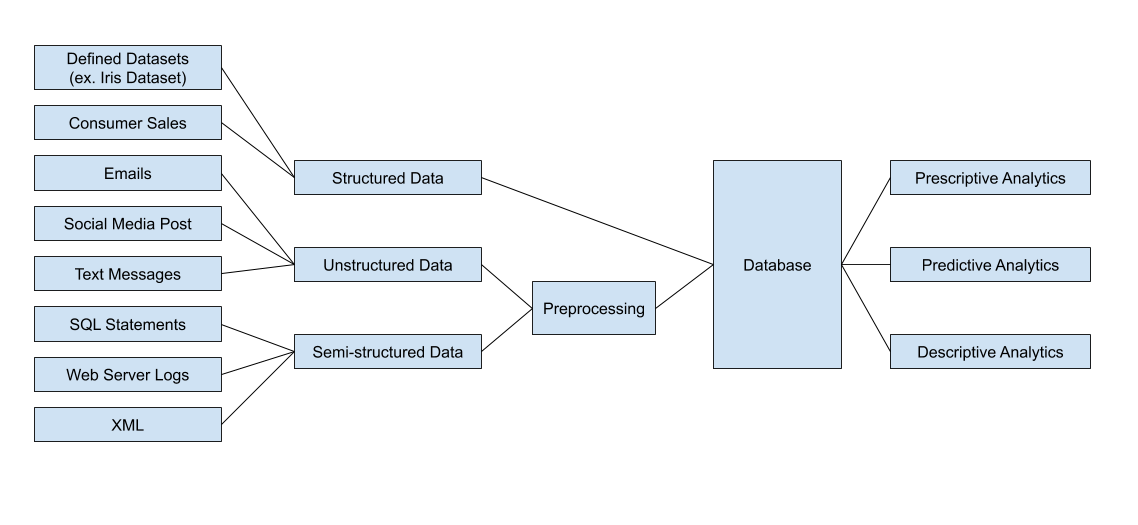
\includegraphics[scale=0.40]{Analytics}
\caption{The relationship between the three types of Big Data and analytics, inspired from the article by S. Jeble, S. Kumari, and Y. Patil \cite{Jeble2016}.}
\end{figure}

\begin{paragraph}
\indent Three forms of analytics can be used on this data stored in the databases which are descriptive, predictive, and prescriptive. Descriptive focuses on the use of information to show relationships between information that occurred within the past \cite{Jeble2016}. Prescriptive analytics is for analyzing data to determine the correct decision to make \cite{Jeble2016}. Predictive analytics is the identification of patterns in data by using statistics and computer science to figure out a solution to a problem. Predictive analytics uses computer algorithms to analyze a set of data, then create conclusions from patterns and relationships that exist between data \cite{Jeble2016}. Predictive analytics is utilized to enable accurate predictions from a given set of data \cite{Jeble2016}. Fig. 2 shows the overall relationship between the various types of big data related to the three forms of analytics.
\end{paragraph}

\subsection{Predictive Analytics and Business}
\begin{paragraph}
\indent Predictive analytics is used in numerous fields, from medicine to retail, as it has the potential to provide insightful information to help people make a well--informed decision about a problem \cite{Jeble2016}. The use of predictive analytics allows businesses to determine the best course of action for marketing campaigns to predicting the sales outcomes of a given product compared to the competition \cite{Jeble2016}. One of the most prevalent practices in business that many online people see is targeted advertisements. The advertisements are chosen based upon the browsing history stored on the user's computer. The purpose of these target ads is to engage the users' interest about a product or service to encourage the purchase of a product from the company; however, stated previously, issues can arise from monitoring and tracking the habits of a user, such as with the use of statistics to predict information.
\end{paragraph}

%--------------------------------------------------------------------------
\section{Making Predictions With Regression}
\begin{paragraph}
\indent One of the biggest purposes of collecting data is to find relationships that occur between data. The concept leads to the use of regression, a topic of statistics, to enable individuals to find the correlation within a set of data. \textit{Linear regression} is used to show the correlation between two variables, one independent and one dependent using a function that best represents the correlation between the two variables with the smallest error between the correlation \cite{Stats2015}. $\hat{y}=\alpha+\beta X$ represents the function used to show the relationship between the two variables of observation \cite{Stats2015}. The linear regression formula is very similar to the slope-intercept form, which is $Y=MX+B$, where $Y$ and $\hat{Y}$ represent the y--coordinate output \cite{Stats2015}. $\alpha$ and $B$ represents the y--intercept point at which the line intersects the y--axis \cite{Stats2015}. The $\beta$ and $M$ variables represent the slope of the function \cite{Stats2015}. The line created from performing linear regression then allows for predictions of future outputs from an input value $X$ \cite{Stats2015}. The example in Fig. 3 shows the use of linear regression on the relationship between blood pressure readings and stress test scores \cite{LinPNG}. The line that bisects the plotted data is the linear regression function is used to make predictions on futures results given a $X$ value along the x--axis for the given set of data.

\begin{figure}[!h]
\centering
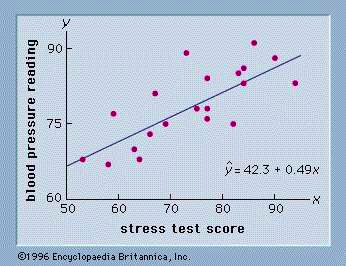
\includegraphics[scale=0.80]{LinReg}
\caption{An example of linear regression showing the correlation between blood pressure readings and stress test scores data \cite{LinPNG}. The x--axis represents stress test scores, and the y--axis is blood pressure readings.}
\end{figure}

\par
\indent The next form of regression used by the researchers during the PNAS study is called logistic regression. \textit{Logistic regression} is a form of regression based upon the probability of an outcome occurring \cite{PrinDS}. The function $p=\frac{e^{\alpha+\beta X}}{1+e^{\alpha+\beta X}}$ represents the logistic regression using parts the linear regression formula in the equation \cite{PrinDS}. The variable $p$ represents the probability of an event occurring \cite{PrinDS}. The component of the function $\alpha+\beta X$ is the linear regression function of a set of data, which is substituted into the logistic regression equation to determine the probability of a $X$ value occurring \cite{PrinDS}. However, there is another form of regression used to make predictions using multiple independent variables.
\par

\begin{figure}[h]
\centering
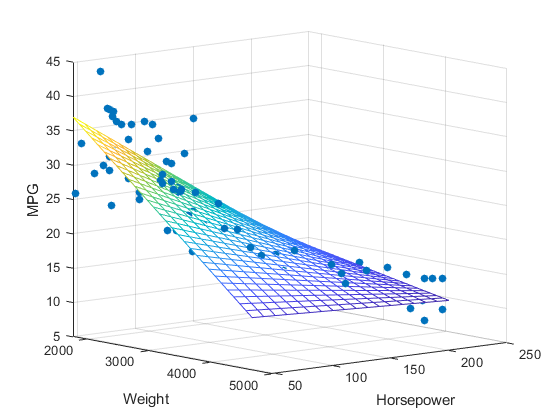
\includegraphics[scale=0.80]{MultiReg}
\caption{Multiple regression plane created from a set of data containing miles per gallon of fuel, vehicle weight, and horsepower \cite{MultiPNG}.}
\end{figure}

\indent Another form of regression called \textit{multiple regression}, which can be used to analyze how multiple independent variables affect a single dependent variable \cite{Stats2015}. The methods for performing multiple regression are similar to linear regression but includes more than one intercept and slope pair in the equation \cite{Stats2015}. Figure 4 shows an example relationship between miles per gallon of gas used, the weight of a vehicle, and vehicle horsepower \cite{MultiPNG}. Similar to linear regression, the line that bisects the points on the three-dimensional graph is the multiple regression function that shows the relationship of the data, which can be of use to make predictions with the data \cite{Stats2015}. One of the significant problems of multiple and linear regression is that only one dependent variable can be interacted with from the provided data. Another way of predicting information has to be used to predict various outputs from a data set.

\end{paragraph}


\section{Machine Learning}
\begin{paragraph}
\indent Machine Learning is a subset field of \textit{artificial intelligence} that specifically focuses on using an algorithm designed to learn and make conclusions from a set of data \cite{pythonML}. There are three types of machine learning: supervised, unsupervised, and reinforcement learning \cite{pythonML}. Supervised learning is a type of machine learning used for predicting outcomes and future information from a well-established correlation between the data as training set of data \cite{pythonML}. Unsupervised learning focuses on looking for hidden structures within a given set of data \cite{pythonML}. Lastly, reinforcement learning is learning through a series of right and wrong actions, like how people learn mathematics \cite{pythonML}. One of the most well--known data set used for machine learning examples is the iris data set. The iris data set is used as a simple data set to teach programmers how to write machine learning code \cite{pythonML}. The iris data set consists of measurements were the sepal length and width along with the petal length and width along with the subspecies name of each of the iris flowers \cite{pythonML}. Each flower within the data set can be known as an instance, object, or set of features \cite{pythonML}. The measurements that make up the flower are known as features \cite{pythonML}. The subspecies names of the flowers are called the class label or targets, which is the value to be predicted \cite{pythonML}.  Before creating a machine learning algorithm, a gasp of what is occurring behind the scenes will help with the understanding of machine learning code as well.
\end{paragraph}

\subsection{The Internal Workings of Machine Learning}
\begin{paragraph}
\indent The way that machine learning makes decisions is by using objects called artificial neurons \cite{pythonML}. The \textit{artificial neurons} are mathematical forms of the \textit{neurons} in the human brain \cite{pythonML}. Two types of neurons exist the \textit{perceptron} and \textit{Adaline}, noted in Fig. 5 \cite{pythonML}.  As humans have a biological brain with many complex structures for processing information, it inspired for an artificial working brain to be recreated using mathematical functions to represent each of the parts of the artificial neuron \cite{pythonML}. The perceptron was published in 1957 by Frank Rosenblatt, which brought the concept to fruition \cite{pythonML}.
\par

\begin{figure}[!hb]
\centering
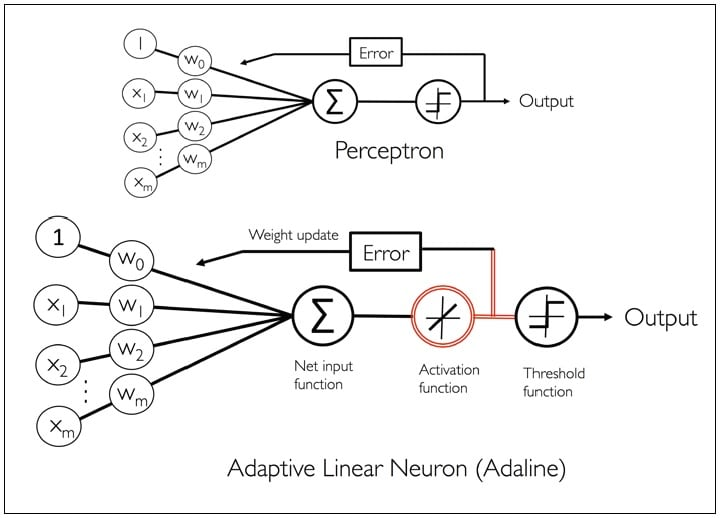
\includegraphics[scale=0.63]{neurons}
\caption{A diagram that shows the structure of the perceptron and Adaline artificial neurons used for machine learning \cite{Neuron}.}
\end{figure}

\indent The first part the perceptron is represented by the variables \(x\) and \(w\) where \(x\) is the input value while \(w\) is referred as the vector weight \cite{pythonML}. The net input is determined by summing the multiplication of the inputs and weights \cite{pythonML}. Once the summation has completed, the neuron will use a threshold function to determine if the neuron will activate or not \cite{pythonML}. The resulting output of the neuron is denoted as \( output^{(i)} \) \cite{pythonML}. If the artificial neuron activates, then the weight is updated by calculating the error and the result outputted \cite{pythonML}. The other form of an artificial neuron, Adaline, which uses an activation function before determining the updated weights and the output of the artificial neuron \cite{pythonML}. The activation function is interchangeable with other functions \cite{pythonML}. The basic example of the two neurons can further be adjusted to hold various threshold and activation functions to represent different models that the artificial neurons are to represent \cite{pythonML}.
\par
\indent Additionally, to further enhance the accuracy of the artificial neuron, multiple iterations over a set of data can be used to keep updating the weights to create an accurate model; with each of these times, the set of data goes through the artificial neuron is called an epoch \cite{pythonML}. After an epoch, the weights update using the various functions depending on the type of artificial neuron used \cite{pythonML}. Just like the human brain, all of the artificial neurons can have connections to other artificial neurons creating a structure that resembles a human brain, which is called an  \textit{ artificial neural network} \cite{pythonML}.
\par

\begin{figure}[!h]
\centering
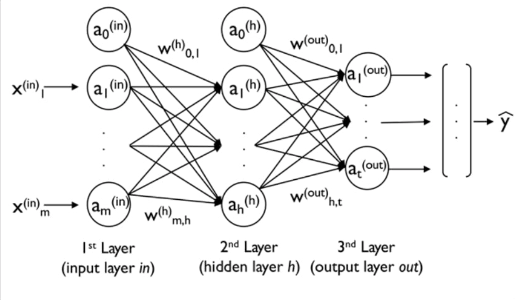
\includegraphics[scale=0.63]{NN}
\caption{A diagram showing the structure of an artificial neural network, using perceptrons, called the mutilayer perceptron \cite{pythonML}.}
\end{figure}

\indent Three layers exist in a multilayer neural network the input layer, hidden layer, and output layer \cite{pythonML}. The input layer is the first set of neurons that interact with the data \cite{pythonML}. The layers after the input layer are called the hidden layer, which can be multiple layers that connect between the input layer and the output layer \cite{pythonML}. The final layer is called the output layer, which is the last layer of the artificial neural network, that outputs the results concluded from the input data \cite{pythonML}. Whenever an artificial neural network has multiple hidden layers, these artificial networks are named deep artificial neural network \cite{pythonML}. One example of an artificial neural network is the multilayer perceptron (MLP), which is a feedforward neural network, meaning that each of the artificial neurons' outputs are inputs for the next layer of neurons \cite{pythonML}. The MLP has to conduct four necessary steps during each epoch to create an accurate model \cite{pythonML}. In the first step, called forward propagation, the data is sent through the neural network to determine an output \cite{pythonML}. In step 2, after determining the output, the error is determined by minimizing the utilization of a \textit{cost function} \cite{pythonML}. The third step is called backpropagation, in short, is finding the derivative of the error using each weight in the model and updating the weights of the model \cite{pythonML}. The first three steps conducted is an epoch and can be repeated multiple times until the final step occurs \cite{pythonML}. Once the number of desired epochs are completed, in the last step, the model can begin making predictions using forward propagation and a threshold function to predict an outcome \cite{pythonML}. However, the artificial neurons and the artificial neuron network are not the only forms of machine learning used to make predictions on a set of data as there are sub--types of machine learning.

\end{paragraph}

\subsection{Sub--types of Machine Learning}

\begin{figure}[!h]
\centering
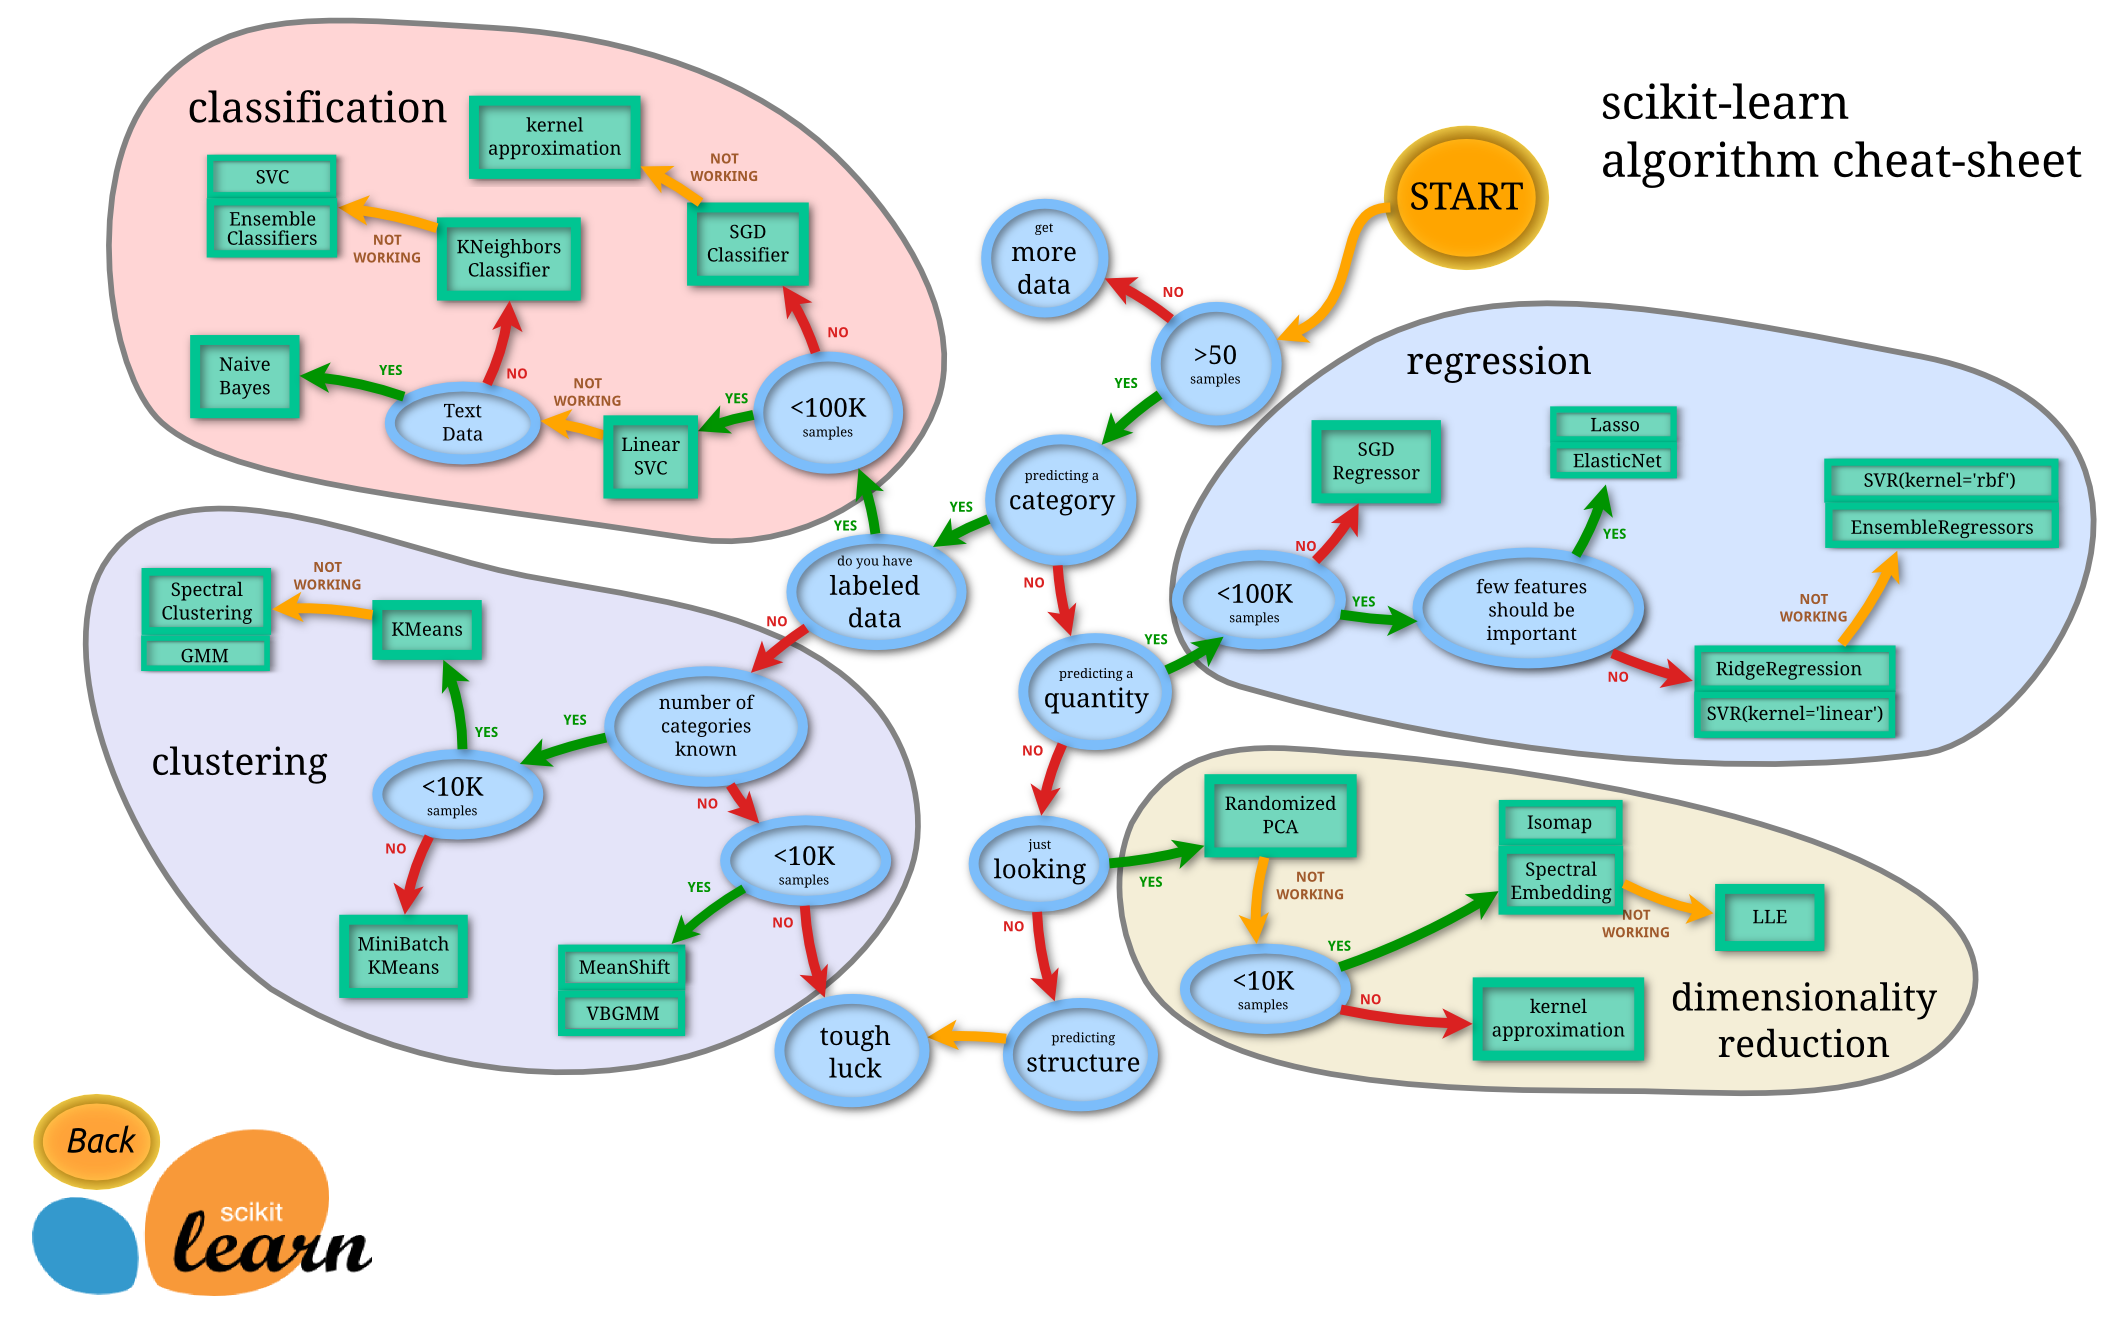
\includegraphics[scale=0.1]{ml_map}
\caption{Map from the scikit--learn website provided to help determine which estimators to use for machine learning \cite{SciKit}.}
\end{figure}

\begin{paragraph}
\indent As there are three types of machine learning, there are a few sub--types of machine learning within every kind of machine learning, which are classification, regression, clustering, and dimensionality reduction \cite{pythonML}. The first form, classification, is a form of machine learning algorithms used to predict an output of one or more features from a set of input data \cite{pythonML}. Regression algorithms make predictions on data from the function that best fit the correlation of data, which is a concept from statistics. Clustering algorithms are used to group data together to find similarities between the elements in the data set, which falls under unsupervised learning \cite{pythonML}. Lastly, dimensionality reduction is an algorithm that shirks the size of a set of data into smaller dimensions \cite{pythonML}. The primary use of dimensionality reduction is to create visualizations of complex graphs of a collection of data \cite{pythonML}. The scikit--learn, library website displays a diagram, Fig. 7, that helps programmers determine the machine learning algorithm that would be best to use \cite{SciKit}. Two libraries exist to work with machine learning algorithms called Scikit--learn (sklearn) and TensorFlow \cite{pythonML}.
\end{paragraph}

\subsection{Scikit-learn vs TensorFlow}
\begin{paragraph}
\indent Two standard libraries and platforms typically used for machine learning with Python are scikit--learn and TensorFlow \cite{pythonML}. Both of the libraries focus on using a machine--learning algorithm to analyze data, but each of the libraries carries out machine learning differently. The scikit--learn library uses pre-created algorithms to create machine learning models. TensorFlow has a similar capability of using the same estimators as scikit--learn but contains other features that make it primarily used for deep learning \cite{pythonML}. TensorFlow can work with a computer's graphics processing unit (GPU), enabling complex computations working with the central processing unit (CPU) \cite{pythonML}. TensorFlow was developed and maintained by Google\textsuperscript{\textregistered} and supports working with CUDA cores that are specific to certain GPUs \cite{pythonML}. Scikit--learn relies solely on using the CPU, which reduces the speed of the computations since parallel processing with the graphics processing unit can not occur \cite{pythonML}. Due to time constraints, Scikit--learn is going to be used as TensorFlow requires more time to be used compared to scikit--learn which was learned about during the early stages of the project \cite{pythonML}.
\end{paragraph}

%--------------------------------------------------------------------------
\section{Machine Learning And Personality Prediction}

\subsection{The Experiment's Plan}
\begin{paragraph}
\indent Now that a general understanding of the topics associated with predicting information, an experiment can be set up to answer the initial question. The experiment will need two essential things to conduct the test: a data set and an algorithm to process and display the information.  A data set can be obtained online from various resources. Once the data set is determined, an algorithm to interact with the data set will be setup. The algorithm will have to be able to compare the results of the machine learning models using standardize variables to show the relationship between the amount of data the models are using to make predictions. Those variables will be total time per set of models, number of features analyzed by the models, and the overall average accuracy score of analyzed models. One of the most important things about the algorithm is to make it easy to understand and only have the estimators and input data be different to ensure that other parts in the code do not affect the final results of the test.
\end{paragraph}

\subsection{The Data Set and Preparation For Testing}
\begin{paragraph}
\indent The chosen data set is a study posted on Kaggle.com, conducted by a statistics class from Comenius University In Bratislava of Slovakian of people between the ages 15 and 30 years old with over 1000 responses\cite{DataSet}. The question within the survey pertained to music, movies, hobbies and interests, phobias, health habits, spending habits, and demographics \cite{DataSet}. The study contains 150 questions overall, with the majority of the items over the topic of personality traits, views on life, and opinions \cite{DataSet}. The majority of the questions are recorded as integers 1 through 4, and others based on category phrases \cite{DataSet}. Before the interaction with the data, a step called preprocessing must occur, which is accomplishable with code; however, the spreadsheet program LibreOffice Calc was used to manually process and organize the data into a usable format. The data set had a few problems to address.
\par
\indent One of the problems within the data set is that some of the values are missing, which were the result of people not answering some of the questions \cite{DataSet}. The missing values are represented by the number 999 as it is not used as an answer for any of the responses. Another issue that arose is that each of the categorical answers use phrases as responses to questions, so they were formatted into a numerical value like the other integer responses. The questions that used these types of responses are health habits questions 1 through 3, question 57 of personality traits, views on life, and opinions, in conjunction with demographic questions 5 through 10 \cite{DataSet}. The phases were changed to integer values 1 through n responses for the given question to simplify the processing by the machine learning algorithm. The last issue to address form the data set is having so many questions that do not pertain to the topic of focus. The number of questions had a reduction to include a single personality trait, anger, and the relationship to the response to all of the spending habits questions.
\par
\indent Lastly, to finish the setup processing of the data before using the machine learning algorithm, the data was put in a format that is usable for making comparisons between the different versions of the machine learning model. As the purpose is to determine whether a person gets angry based on spending habits, the spending habits questions where further subdivided to see the relationship between the number of features to the target feature anger to be predicted. Seven CSV files were used, starting with one feature and the target feature until there where seven features and one target feature. Doing this allows the algorithm to be set up in a way that will enable a more straightforward analysis.
\end{paragraph}

\subsection{The Algorithm}
\begin{paragraph}
\indent One of the biggest challenges for machine learning is picking the proper estimator to work with as there are numerous ways of analyzing the data set. The scikit--learn website has a diagram that helps guide the best machine learning models are best to use, noted in Fig. 7 \cite{SciKit}. The diagram recommends using the algorithms SVM and KNearestNeighbor but ultimately decided to use their version of the multilayer perceptron called the MLPClassifer, not listed on the diagram \cite{SciKit}. The selection of the MLPClassifer ultimately leads up to the final algorithm after numerous instances of tinkering with the machine--learning code. The code was inspired from a sample set by Jason Brownlee from machinelearningmastery.com that is used on the iris data set \cite{MLMaster}. The inspiration from Brownlee and scikit--learn lead to the following code to be developed. 

\par
\indent The first part of the algorithm, located below in lines 4 through 28, is the Local Declarations inside of the main functions that have multiple arrays initialized for storing and plotting the results from creating and make predictions with the models. The average number of models to analyze is 10 models per set of features observed. The next section, which is under Local Statements, is Data Handling. The first part is initial print statements to tell the user what the program is doing. The first for loop, at line 39, is used to iterate between the models to be compared. The next loop, line 42, is to iterate over the different CSV files, located in if statements in lines 45 through 198, that store the data sets for training and validation. Each of the if statements load the data from a CSV file, then initializes an array that are the labels of the features. The data is then stored into a large array to be further split into an array of X features and targets to predict y. The function\texttt{ train\_test\_split} to split the data into a training and validation set with 20 percent used for validation and 80 percent for training. The steps, in the if statements, will be used each time to train a new set of models, which leads into the section of the code called Model Creation and Prediction.
\newline
\begin{lstlisting}[frame = single]
#Main Function ----------------------------------------------------------------
def main():

    #Local Declarations -----------------------------------

    #Initialization of variables
    average = 10              #Number of times to make a model to determine
                              # overall average accuracy score

    feature = [1,2,3,4,5,6,7] #List of the amount of features used per model

    MLPdata1 = []             #List to store overall average accuracy
                              # of MLPClassifier

    MLPdata2 = []             #List to store overall average accuracy
                              # of MLPClassifier

    MLPdata3 = []             #List to store overall average accuracy
                              # of MLPClassifier

    final_time1 = []          #List to store time taken to analyze both models
                              # with n features

    final_time2 = []          #List to store time taken to analyze both models
                              # with n features

    final_time3 = []          #List to store time taken to analyze both models
                              # with n features
    
    #Local Statements -------------------------------------

    #SECTION: Data Handling----------------------------------------------------

    print("        MLPClassifier Model Comparison         ")
    print("-----------------------------------------------")
    print("Please wait until the 3D scatter plot displays ")

    #For loop to iterate through all models being observed
    for iter_selection in range(3):
  
        #For loop to iterate through data sets used by the models and estimators
        for i in range(7):

            #If statements to that determine which set of data is being used
            if i == 0:
                #Load data set values from CSV file
                csvData = "responses-1feature-finances.csv"
                
                #Array to store names of feature(s) and target feature
                names = ['Getting angry', 'Finances']

                #Stores the data values with names of questions
                dataset = read_csv(csvData, names=names)

                #Stores array values into an array
                array = dataset.values

                #Initialization of two NumPy X and y arrays
                X1 = array[:,0:2]
                y1 = array[:,0]

                #Function to split the question values into a training set where 20 percent of the 
                # data set is used for validation
                (X_train, X_validation, Y_train, Y_validation) = train_test_split(X1, y1, test_size=0.20)

\end{lstlisting}
\textbf{Note:} The remainder of this section can be found in the appendix of the paper that contains the entire algorithm.
\newline

\par
\indent In the Model Creation and Predictions section, the models are created, validated, and their results stored in this section of the code. A nested for loop, below starting at line 13, is used to iterate ten times over the estimators that contain parameters for each model to be made. The first step, in line 5 is to initialize the variable that stores the average accuracy for each test to prevent extra data inclusion in another test. The time method and function, \texttt{tm.time()}, line 11, is then used to take the current time on the computer, which will be used to determine the amount of time taken. Within the loop are if statements, lines 15, 20, and 25, that determines which models are going to be made. The MLPClassifier function contains the parameters and runs through the scikit--learn's algorithm for the multilayer perceptron. The MLPClassifier has 23 parameters that can be tweaked to build models for making predictions on a given data set \cite{SciKit}. The MLPClassifier estimator can use three solvers, quasi-Newton methods, stochastic gradient descent, and stochastic gradient-based optimizer used to update the weights of the neurons within the artificial neural network \cite{SciKit}. The solvers also have parameters to be passed that changes the settings of the solvers as well. Then the function called \texttt{fit}, line 31, is used to train the artificial neural network using the passed parameters of the estimator and the two input arrays that contain the training data. Once the training is complete, the \texttt{predict} method, line 34, is used to validate the model using the validation set of data. The results of the model, when compared to the known target validation data using the \texttt{accuracy\_score} function, line 37, which will return the accuracy score of the model. The time function is used again, at line 40 after all of the models' creation and validation, to calculate the total time taken to calculate the average accuracy score of all of the models. Once the calculations are complete, the results are appended into arrays, lines 46 through 70, that are specific to the estimator used to make the models to be later graphed. The process repeats until all estimators iterated over and set of features are analyzed.
\newline
\begin{lstlisting}[frame = single]
    #Section: Model Creation and Prediction------------------------------------

            #Sets the overall average accuracy to zero before each test
            # extra information is not used is the next test's results
            MLPavg = 0

            #https://scikit-learn.org/stable/index.html
            #Initialization of the model to be used along with parameters to use

            #Time function to begin timer
            start_time = tm.time()

            for i in range(average):

                if iter_selection == 0:

                    #Default MLPClassifier
                    estimator_MLP = MLPClassifier(max_iter=1400)

                if iter_selection == 1:

                    #MLPClassifier with tangent activation function
                    estimator_MLP = MLPClassifier(activation='tanh', max_iter=1400)

                if iter_selection == 2:

                    #MLP Classifier with logistic activation function
                    estimator_MLP = MLPClassifier(activation='logistic', max_iter=1400)

                #Function to train the model with the data set
                estimator_MLP.fit(X_train, Y_train)

                #Prediction function for MLPClassifer
                prediction_MLP = estimator_MLP.predict(X_validation)
               
                #Determine the accuracy score of the model
                MLPavg = accuracy_score(Y_validation, prediction_MLP) * 100 + MLPavg

            #Takes and stores the stop time of determining the model average
            stop_time = tm.time() - start_time
            
            #Determines the average overall accuracy
            MLPavg = MLPavg / average

            #Stores the information of the first model
            if iter_selection == 0:   
                
                #Stores accuracy results of test into an array
                MLPdata1.append(float(MLPavg))

                #Stores time results of test in an array
                final_time1.append(float(stop_time))

            #Stores the information of the second model
            if iter_selection == 1:

                #Stores accuracy results of test into an array
                MLPdata2.append(float(MLPavg))

                #Stores time results of test in an array
                final_time2.append(float(stop_time))

            #Stores the information of the third model
            if iter_selection == 2:

                #Stores accuracy results of test into an array
                MLPdata3.append(float(MLPavg))

                #Stores time results of test in an array
                final_time3.append(float(stop_time))
\end{lstlisting}

\par

\indent The last section called Displaying Results plots the data stored in the arrays into a three-dimensional scatter plot that shows the three observed variables number of features, overall average accuracy, and time. The reason the scatter plot was chose is to show all three variables relationship with each other. The library used to create the scatter plots was MatPlotLib, which has various assortments of graphics used to display data. The first function, listed below in line 4, is used to determine which type of graphic is going to be used to display the data. The next three functions, lines 7 through 10, plot the data, which are lists that contain the data from the earlier test. The feature list only contains the integers one through seven, highlighting the number of features used to make predictions. The rest of the functions, lines 13 through 17, are for labeling the diagram to display the table and axis labels. The whole process took awhile various issues occurred with the algorithm, such as convergence warnings where the solvers were not reaching their full potential and revisions to make the algorithm work as flawless as possible.
\newline
\begin{lstlisting}[frame = single]
    #Section: Displaying Results-----------------------------------------------

    #Initialization of MatPlotLib model
    ax = plt.axes(projection='3d')

    #Plots MLPClassifier data
    ax.scatter3D(feature, MLPdata1, final_time1)
    ax.scatter3D(feature, MLPdata2, final_time2)
    ax.scatter3D(feature, MLPdata3, final_time3)
    ax.legend(['Default','Tangent','Logistic'])

    #Axis labels and figure title
    ax.set_xlabel('Number Of Features')
    ax.set_ylabel('Average Accuracy Score')
    ax.set_zlabel('Time Taken (Seconds)')
    title = 'MLPClassifier Average of ' + str(average) + ' Model(s)'
    ax.set_title(title)

    #Shows graph to screen
    plt.show()
    
#Main function call------------------------------------------------------------
main()
\end{lstlisting}

\end{paragraph}

\subsection{The Experiment}
\begin{paragraph}
\indent The experiment will have three tests with the algorithm, and then the tests are compared. Each of the MLPClassifer parameters will be different for the three estimators. The first estimators will have all default parameters outlined on the scikit--learn's website except for the max number of iterations. The max number of iterations across all estimators is at 1400 epochs. The reason this is done because of convergence problems with the estimators were not reaching the most optimized point with the weight solvers to create models with the most optimum weights. The second estimator will use the same parameters as the first model with only one exception; the activation function is configured to tangent. The last estimator follows suit with the previous estimator but uses the logistic activation function instead. Once the testing of the models finishes, all three estimators' results will then be plotted on a scatter plot together for comparing the differences. My initial predictions for the outcomes of the models, whereas the number of features increases, the average overall accuracy will increase. Also, as the number of features increase, the time taken to create and make predictions with the set of models will grow as well, but the results from the three test display otherwise.
\end{paragraph}

\subsection{The Results}
\begin{figure}[h]
\centering
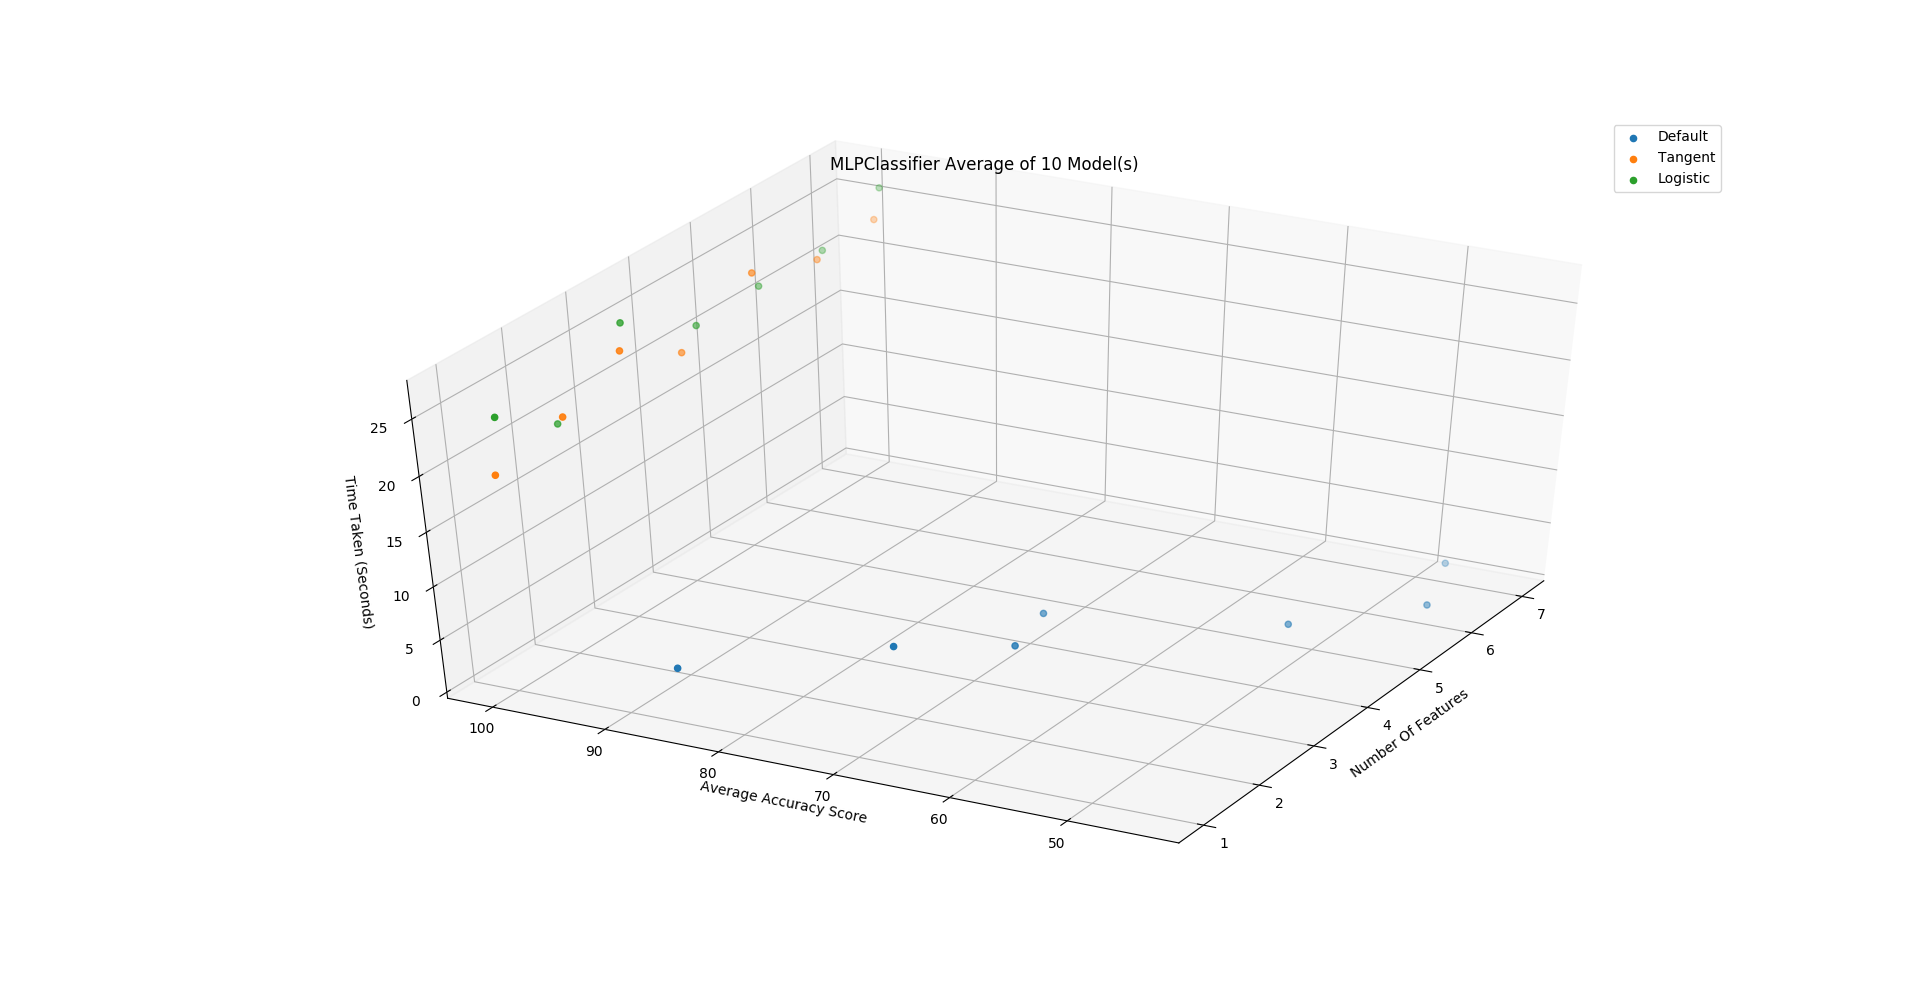
\includegraphics[scale=0.37]{Test_1}
\caption{The results of the first test results of the MLPClassifer Comparison algorithm. X--axis is Number of Features, Y--axis is average accuracy score, and Z--axis is Time Taken in seconds.}
\end{figure}
\begin{paragraph}
\indent The results for the first test,noted in Fig. 8, shows contrary to my initial assumption about the performance of the models. The first model, called Default, first average with one feature obtained an average accuracy score of over 90 percent and less than five seconds to process. As the number of features increased, the time taken remained similar; however, the average accuracy score has a decreasing trend from one feature models. The trend lasted until the lowest scores were between 50 and 40 percent with the 6 and 7 feature models, with six feature models appearing close to a 45 percent as the average accuracy score. The other two estimators, called Tangent and Logistic have a similar correlation of results. The Tangent models appear to have an average accuracy score of over 95 percent across all models created. Along with both of the models Time between 25 to 15 seconds for creation and prediction of the models.
\par

\begin{figure}[!h]
\centering
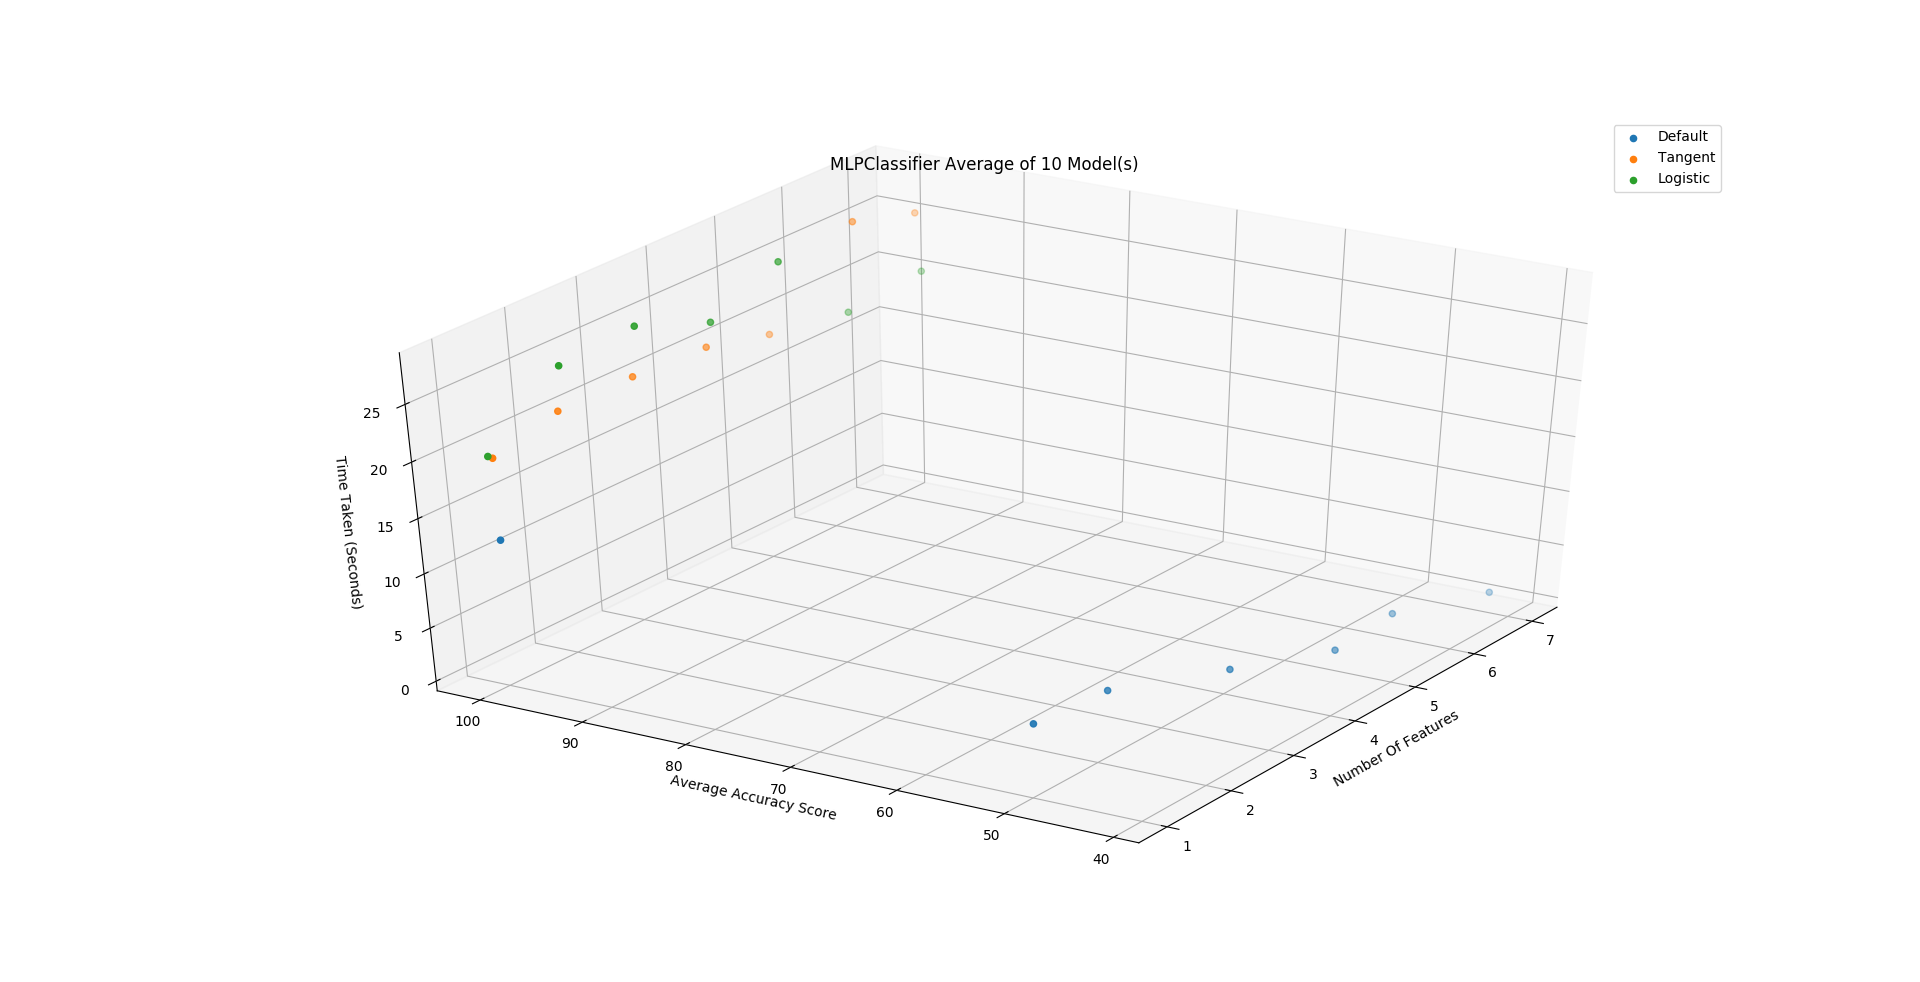
\includegraphics[scale=0.37]{Test_2}
\caption{ The results of the second test results of the MLPClassifer Comparison algorithm. X--axis is Number of Features, Y--axis is average accuracy score, and Z--axis is Time Taken in seconds.}
\end{figure}

The second test, Fig. 9, was similar to the first test, with the Default models having a decreasing trend. The models with one feature having an average accuracy score of at least 95 percent than with the next dropping to below 60 percent, and the results continuously decreasing until the seven feature models with an average accuracy score between 45 and 40 percent. The times for the Default models range from at most 15 seconds to less than five seconds, with one feature models being the highest and the seven feature models being the lowest. The Tangent and Logistic models again show a close correlation, but the logistics functions having taken longer to be created and validated until models with six and seven features. The two adjusted models also appear again to have an average accuracy score of at least 95 percent.
\par

\begin{figure}[h]
\centering
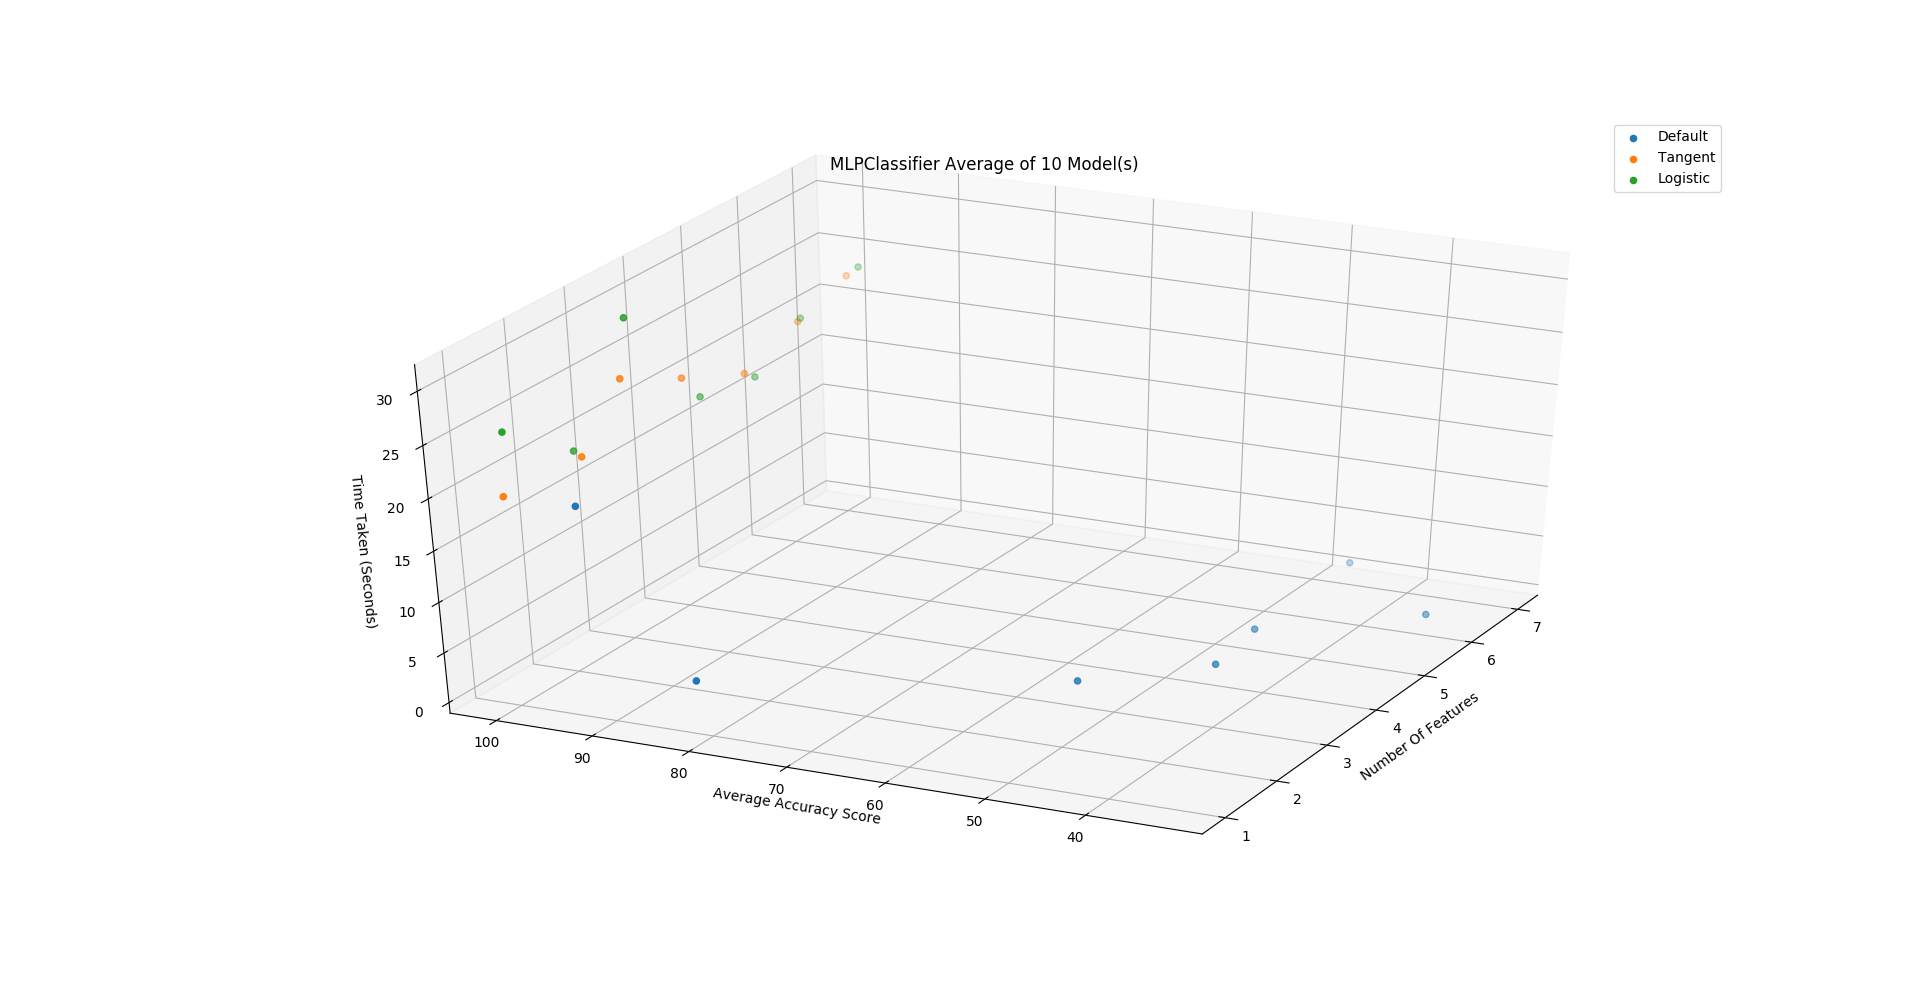
\includegraphics[scale=0.37]{Test_3}
\caption{The results of the third test results of the MLPClassifer Comparison algorithm. X--axis is Number of Features, Y--axis is average accuracy score, and Z--axis is Time Taken in seconds.}
\end{figure}

The third and last test, Fig. 10, has more variation compared to the two previous tests. The Default models had an overall average accuracy score for one feature models of at least 85 percent then increases with two feature models reaching above 95 then for the rest of the Default models, decreasing to below 60 percent for the remainder of the sets of models. The most time used of the Default models is the two feature models with between 15 and 10 seconds total time taken to create and validate with models and all other models having times less than five seconds. The Tangent and Logistic models correlated closely together again with the first three sets of Logistic models having higher total creation and validation times than the Tangent models, and then following closely with the Tangent models between 15 and 20 seconds to create and validate the models. The three feature Logistic models had the highest run-time with more than 25 seconds to generate and validate the models.

\par
Out of all three tests combined, the Tangent and Logistic models had higher average accuracy score but took more time to create and validate the models. The Default models were sporadic, with the majority of the one feature average accuracy scores being above at least 80 percent. Based on the results of the three tests, the personality of a person with one feature is predictable using a multilayer perceptron classifier. For the models to have better overall average accuracy, the estimators must be tuned and tested to have the models make accurate predictions about a personality trait of a person. My initial assumptions about the results turned out to be slightly different. With the average accuracy score decreasing as the number of features increased for the Default models and the Tangent and Logistic Models were very similar and had high average accuracy scores for all tests.
\end{paragraph}

\section{Future Works}
\begin{paragraph}
\indent Given the results and concepts learned from the project, many other aspects could have been included in the project. All parameters of the MLPClassifer could have been tested during the project, like the effects of tolerances on models. The project could have more depth by observing every process of multiple machine learning algorithms in exquisite detail, outlining the many mathematical algorithms that enable machine learning to work. Aside from using the MLPClassifer to analyze the data set, other types and sub-types of machine learning could have been used to investigate the data further and make conclusions from the data. The overall limiting factor of the project is the time constraint of the project being a single semester. The work can be further built upon to analyze the data set or continue learning about the topic of machine learning.
\end{paragraph}

\section{Conclusion}
\begin{paragraph}
\indent In conclusion, the project's goal was to use online data to demonstrate that using a limited amount of information can lead to uncovering private details about an individual. The project successfully demonstrates using a machine learning algorithm; only one feature is needed to predict the personality trait of a given person accurately. The goal was accomplished by fine-tuning of the parameters of the estimators can increase the accuracy score of the models with allowing for accurate predictions to occur from a set of data. The details that go into ways for predictive analytics are very expansive, with numerous paths and fine details to consider before going deep into predictive analytics as small changes can lead to significant differences in outcomes. The broadness of predictive analytics implies that many industries use analytics for different purposes but use similar programming techniques to accomplish their individual goals. The research shows that there is a complicated relationship between disciplines and sectors. The research and details could have gone extremely in-depth due to time constraints of the semester and provided clarity, some details about the various subjects discussed where not covered extensively. A lot more time could have a focus on analyzing every parameter that affects the output of the classifiers but had to have a reduction to just three to four changes of the estimator. More time could be on building and conducting a custom survey, but again time was against the project. The biggest take away from the project that self-learning, self-disciple, and practice can allow for new exciting things to be self-taught. And always do extensive research to learn about a subject as the tools can be of use to further a goal or objective later down the road.
\end{paragraph}

\newpage
\section{Appendix: Definitions}
\begin{itemize}
\item[]
\textit{Linear regression} -- A statistics concept used to show the correlation between two variables, one independent and one dependent using a function that best represents the correlation between the two variables with the smallest error between the correlation, $\hat{y}=\alpha+\beta X$ \cite{Stats2015}.
\item[]
\textit{Logistic regression}-- A form of regression based upon the probability of an outcome occurring, $p=\frac{e^{\alpha+\beta X}}{1+e^{\alpha+\beta X}}$ \cite{PrinDS}.
\item[]  
\textit{Singular value decomposition} -- A process in linear algebra to simplify the calculation of a matrix \cite{SVD}.
\item[]
\textit{Big data} -- The mass collection of  data for the purpose of research for by scientist,  government officials, and commercial institutions.
\item[]
\textit{Analytics} -- The analysis of a set of data. 
\item[]
\textit{Multiple regression} -- A statistics concept used to show the correlation between multiple independent and one dependent variables using a function that best represents the correlation \cite{Stats2015}.
\item[]
\textit{Artificial intelligence} -- A concept that a program that is capable of learning and making decisions without human interaction.
\item[]
\textit{Artificial neuron} -- A mathematical form of the neurons found in a biological brain \cite{pythonML}.
\item[]
\textit{neuron} -- A biological component of a brain that sends signals through the brain.
\item[]
\textit{Perceptron} -- A type of artificial neuron that updates its weight after determining the output, and does not contain an activation function within the artificial neuron \cite{pythonML}.
\item[]
\textit{Adaline} -- A type of artificial neuron that updates its weight after an activation function, and before being determining to output or not \cite{pythonML}.
\item[]
\textit{Artificial neural network} -- A interconnection of artificial neurons where their outputs are inputs for the the next layer of artificial neurons \cite{pythonML}.
\item[]
\textit{Cost function} -- A function that  determines how well a machine learning model is performing \cite{Cost}.

\end{itemize}

\newpage
\section{Appendix: Project Program}

\begin{lstlisting}[frame = single]
#Libraries---------------------------------------------------------------------

#Used in Section: Data Handling
from pandas import read_csv
from sklearn.model_selection import train_test_split

#Used in Section: Model Creation and Prediction
from sklearn.metrics import accuracy_score
from sklearn.neural_network import MLPClassifier
import time as tm

#Used in Section: Display Results
from mpl_toolkits import mplot3d
import matplotlib.pyplot as plt

#Main Function ----------------------------------------------------------------
def main():

    #Local Declarations -----------------------------------

    #Initialization of variables
    average = 10              #Number of times to make a model to determine
                              # overall average accuracy score

    feature = [1,2,3,4,5,6,7] #List of the amount of features used per model

    MLPdata1 = []             #List to store overall average accuracy
                              # of MLPClassifier

    MLPdata2 = []             #List to store overall average accuracy
                              # of MLPClassifier

    MLPdata3 = []             #List to store overall average accuracy
                              # of MLPClassifier

    final_time1 = []          #List to store time taken to analyze both models
                              # with n features

    final_time2 = []          #List to store time taken to analyze both models
                              # with n features

    final_time3 = []          #List to store time taken to analyze both models
                              # with n features
    
    #Local Statements -------------------------------------

    #SECTION: Data Handling----------------------------------------------------

    print("        MLPClassifier Model Comparison         ")
    print("-----------------------------------------------")
    print("Please wait until the 3D scatter plot displays ")

    #For loop to iterate through all models being observed
    for iter_selection in range(3):
  
        #For loop to iterate through data sets used by the models and estimators
        for i in range(7):

            #If statements to that determine which set of data is being used
            if i == 0:
                #Load data set values from CSV file
                csvData = "responses-1feature-finances.csv"
                
                #Array to store names of feature(s) and target feature
                names = ['Getting angry', 'Finances']

                #Stores the data values with names of questions
                dataset = read_csv(csvData, names=names)

                #Stores array values into an array
                array = dataset.values

                #Initialization of two NumPy X and y arrays
                X1 = array[:,0:2]
                y1 = array[:,0]

                #Function to split the question values into a training set where 20 percent of the 
                # data set is used for validation
                (X_train, X_validation, Y_train, Y_validation) = train_test_split(X1, y1, test_size=0.20)

            if i == 1:
                #Load data set values from CSV file
                csvData = "responses-2features.csv"    

                #Array to store names of feature(s) and target feature
                names = ['Getting angry', 'Finances','Shopping centres']
    
                #Stores the data values with names of questions
                dataset = read_csv(csvData, names=names)

                #Stores array values into an array
                array = dataset.values

                #Initialization of two NumPy X and y arrays
                X2 = array[:,0:3]
                y2 = array[:,0]

                #Function to split the question values into a training set where 20 percent of the 
                # data set is used for validation
                (X_train, X_validation, Y_train, Y_validation) = train_test_split(X2, y2, test_size=0.20)

            if i == 2:
                #Load data set values from CSV file
                csvData = "responses-3features.csv"    

                #Array to store names of feature(s) and target feature
                names = ['Getting angry', 'Finances','Shopping centres', 'Branded clothing']
    
                #Stores the data values with names of questions
                dataset = read_csv(csvData, names=names)

                #Stores array values into an array
                array = dataset.values

                #Initialization of two numpy X and y arrays
                X3 = array[:,0:4]
                y3 = array[:,0]

                #Function to split the question values into a training set where 20 percent of the 
                # data set is used for validation
                (X_train, X_validation, Y_train, Y_validation) = train_test_split(X3, y3, test_size=0.20)

            if i == 3:

                #Load data set values from CSV file
                csvData = "responses-4features.csv"

                #Array to store names of feature(s) and target feature
                names = ['Getting angry', 'Finances','Shopping centres', 'Branded clothing','Entertainment spending']
    
                #Stores the data values with names of questions
                dataset = read_csv(csvData, names=names)

                #Stores array values into an array
                array = dataset.values

                #Initialization of two numpy X and y arrays
                X4 = array[:,0:5]
                y4 = array[:,0]

                #Function to split the question values into a training set where 20 percent of the 
                # data set is used for validation
                (X_train, X_validation, Y_train, Y_validation) = train_test_split(X4, y4, test_size=0.20)

            if i == 4:

                #Load data set values from CSV file
                csvData = "responses-5features.csv"    

                #Array to store names of feature(s) and target feature
                names = ['Getting angry', 'Finances','Shopping centres', 'Branded clothing',
                         'Entertainment spending', 'Spending on looks']
    
                #Stores the data values with names of questions
                dataset = read_csv(csvData, names=names)

                #Stores array values into an array
                array = dataset.values

                #Initialization of two numpy X and y arrays
                X5 = array[:,0:6]
                y5 = array[:,0]

                #Function to split the question values into a training set where 20 percent of the 
                # data set is used for validation
                (X_train, X_validation, Y_train, Y_validation) = train_test_split(X5, y5, test_size=0.20)

            if i == 5:

                #Load data set values from CSV file
                csvData = "responses-6features.csv"    

                #Array to store names of feature(s) and target feature
                names = ['Getting angry', 'Finances','Shopping centres', 'Branded clothing',
                        'Entertainment spending', 'Spending on looks', 'Spending on gadgets']
    
                #Stores the data values with names of questions
                dataset = read_csv(csvData, names=names)

                #Stores array values into an array
                array = dataset.values

                #Initialization of two numpy X and y arrays
                X6 = array[:,0:7]
                y6 = array[:,0]

                #Function to split the question values into a training set where 20 percent of the 
                # data set is used for validation
                (X_train, X_validation, Y_train, Y_validation) = train_test_split(X6, y6, test_size=0.20)

            if i == 6:

                #Load data set values from CSV file
                csvData = "responses-7features.csv"    

                #Array to store names of feature(s) and target feature
                names = ['Getting angry', 'Finances','Shopping centres', 'Branded clothing',
                         'Entertainment spending', 'Spending on looks', 'Spending on gadgets',
                         'Spending on healthy eating']
    
                #Stores the data values with names of questions
                dataset = read_csv(csvData, names=names)

                #Stores array values into an array
                array = dataset.values

                #Initialization of two numpy X and y arrays
                X7 = array[:,0:8]
                y7 = array[:,0]

                #Function to split the question values into a training set where 20 percent of the 
                # data set is used for validation
                (X_train, X_validation, Y_train, Y_validation) = train_test_split(X7, y7, test_size=0.20)

    #Section: Model Creation and Prediction------------------------------------

            #Sets the overall average accuracy to zero before each test
            # extra information is not used is the next test's results
            MLPavg = 0

            #https://scikit-learn.org/stable/index.html
            #Initialization of the model to be used along with parameters to use

            #Time function to begin timer
            start_time = tm.time()

            for i in range(average):

                if iter_selection == 0:

                    #Default MLPClassifier
                    estimator_MLP = MLPClassifier(max_iter=1400)

                if iter_selection == 1:

                    #MLPClassifier with tangent activation function
                    estimator_MLP = MLPClassifier(activation='tanh', max_iter=1400)

                if iter_selection == 2:

                    #MLP Classifier with logistic activation function
                    estimator_MLP = MLPClassifier(activation='logistic', max_iter=1400)

                #Function to train the model with the data set
                estimator_MLP.fit(X_train, Y_train)

                #Prediction function for MLPClassifer
                prediction_MLP = estimator_MLP.predict(X_validation)
               
                #Determine the accuracy score of the model
                MLPavg = accuracy_score(Y_validation, prediction_MLP) * 100 + MLPavg

            #Takes and stores the stop time of determining the model average
            stop_time = tm.time() - start_time
            
            #Determines the average overall accuracy
            MLPavg = MLPavg / average

            #Stores the information of the first model
            if iter_selection == 0:   
                
                #Stores accuracy results of test into an array
                MLPdata1.append(float(MLPavg))

                #Stores time results of test in an array
                final_time1.append(float(stop_time))

            #Stores the information of the second model
            if iter_selection == 1:

                #Stores accuracy results of test into an array
                MLPdata2.append(float(MLPavg))

                #Stores time results of test in an array
                final_time2.append(float(stop_time))

            #Stores the information of the third model
            if iter_selection == 2:

                #Stores accuracy results of test into an array
                MLPdata3.append(float(MLPavg))

                #Stores time results of test in an array
                final_time3.append(float(stop_time))

    #Section: Displaying Results-----------------------------------------------

    #Initialization of MatPlotLib model
    ax = plt.axes(projection='3d')

    #Plots MLPClassifier data
    ax.scatter3D(feature, MLPdata1, final_time1)
    ax.scatter3D(feature, MLPdata2, final_time2)
    ax.scatter3D(feature, MLPdata3, final_time3)
    ax.legend(['Default','Tangent','Logistic'])

    #Axis labels and figure title
    ax.set_xlabel('Number Of Features')
    ax.set_ylabel('Average Accuracy Score')
    ax.set_zlabel('Time Taken (Seconds)')
    title = 'MLPClassifier Average of ' + str(average) + ' Model(s)'
    ax.set_title(title)

    #Shows graph to screen
    plt.show()
    
#Main function call------------------------------------------------------------
main()
\end{lstlisting}

\newpage
\begin{thebibliography}{99}

\bibitem{IntStats}
M. Roser, H. Ritchie, and E. Ortiz-Ospina (2020),
\say{Internet}. Published online at OurWorldInData.org. Retrieved from: 'https://ourworldindata.org/internet' [Website]

\bibitem{Kosinski2013}
M. Kosinski, D. Stillwell, and T. Graepel (2013),
\say{Private traits and attributes are predicatable from digital records of human behavior}, \textit{PNAS} 110. 15. , 5802 - 5805. Google Scholar. Accessed January 19th 2020 URL: https://www.pnas.org/content/pnas/110/15/5802.full.pdf [Journal]

\bibitem{Jeble2016}
S. Jeble, S. Kumari, and Y. Patil (2016),
\say{Role of big data and predictive analytics}. \textit{International Journal of Automation and Logistics}. 2. 307-331. 10.1504/IJAL.2016.10001272. Google Scholar. Accessed January 21st 2020 URL: https://www.researchgate.net/publication/309809606 [Journal]

\bibitem{Stats2015}
J. Bothe, J. L. Brudney, and K. J. Meier (2015), 
\textit{Applied Statistics For Public and Nonprofit Administration}. 4th ed. Stamford, CT USA Cengage Learning. [eBook]

\bibitem{pythonML}
V. Mirjalili and S. Raschka (2017),
\textit{Python Machine Learning}. 2nd ed. Birmingham, UK Packt Publishing. [eBook]

\bibitem{IrisData}
\say{Iris Data Set'}, University of California Irvine Machine Learning Repository. Accessed February 5th 2020 URL: https://archive.ics.uci.edu/ml/datasets/iris [Website]

\bibitem{DataSet}
M. Sabo (2016), \say{2013 Young People Survey}. Accessed February 13th 2020 URL: https://www.kaggle.com/miroslavsabo/young-people-survey [Website]

\bibitem{SciKit}
\say{scikit-learn Machine Learning in Python}. Accessed February 17th 2020 URL: https://scikit-learn.org/stable/index.html [Website]

\bibitem{Neuron}
www.simplilearn.com (n.d),
\say{How to Train an Artificial Neural Network}. Accessed April 13th 2020 URL: https://www.simplilearn.com/how-to-train-artificial-neural-network-tutorial [Online Image]

\bibitem{PrinDS}
S. Kakade, S. Ozdemir, and M. Tibaldeschi (2018),
\textit{Principles of Data Science}. 2nd ed. Birmingham, UK Packt Publishing Ltd. [eBook]

\bibitem{LinPNG}
D. Anderson, D. Sweeney, and T. Williams (2020),
\say{Statistics}, Encyclopaedia Britannica. Accessed March 23rd 2020 
URL: https://www.britannica.com/science/statistics/Experimental-design\#ref367488 [Online Image]

\bibitem{MultiPNG}
\say{regress} (n.d), MathWorks. Accessed March 23rd 2020 URL: https://www.mathworks.com/help/stats/regress.html [Online Image]

\bibitem{SVD}
J. Brownless (2018),
\say{How to Calculate the SVD from Scratch with Python}. Accessed March 30th 2020 URL: https://machinelearningmastery.com/singular-value-decomposition-for-machine-learning/ [Website]

\bibitem{Cost}
K. Krzyk (2018),
\say{Coding Deep Learning for Beginners Linear Regression (Part 2): Cost Function}. Accessed March 30th 2020 URL: https://towardsdatascience.com/coding-deep-learning-for-beginners-linear-regression-part-2-cost-function-49545303d29f [Website]

\bibitem{MLMaster}
J. Brownlee (2020),
\say{Your First Machine Learning Project in Python Step-By-Step}. Accessed February 5th 2020 URL: https://machinelearningmastery.com/machine-learning-in-python-step-by-step/ [Website]


\end{thebibliography}

\end{document}